\documentclass[12pt,fleqn]{article}\usepackage{../../common}
\begin{document}
Sonlu Öğeler Metotu (Finite Elements Method -FEM-) - 2

Önceki örnekler standart eni değişmeyen kiriş yapısını temel aldı.  Fakat ya
kiriş alttaki gibi olsaydı?

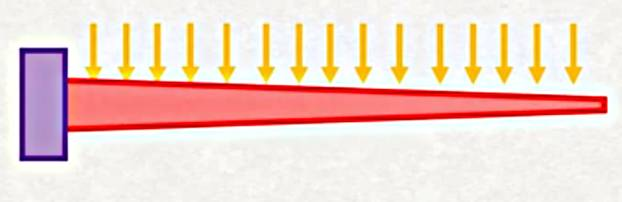
\includegraphics[width=15em]{compscieng_bpp45fem2_01.jpg}

Bu kirişi temsilen

$$
E I \frac{\ud^4 y}{\ud X_1^4} = q
$$

diferansiyel denklemini hala kullanabilir miyiz? Dikkat edersek en değiştiğine
göre $X_1$ ile beraber, ona bağlı olarak, atalet momenti $I$ sabit değil,
değişken demektir.. Bazıları düşünebilir ``ama o zaman değişken $I$'yi alırız,
üstteki denklemdeki $I$'ya sokarız olur biter''. Bunu yapamayız çünkü $I$'nin
sabit olması üstteki denklemi türetmek için bir önkabuldu, yani $I$ değişken ise
üstteki denklemi kullanmak mümkün değildir [1, Ders 4].

Problem şu ki pek çok gerçek dünya uygulaması üstteki Euler-Bernoulli kiriş
formülüne erişirken kullandığımız faraziyelere uymaz, bunları hatırlarsak lineer
elastiklik, yok sayılabilecek Poisson etkileri, düzlemlerin düz kalması idi.
Fakat mesela beton materyelini ele alalım, bu materyel ucuzdur, basınca, yani
içe doğru strese karşı çok dayanıklıdır, ki bu yüzden pek çok yapıda kullanılır,
fakat beton dışa doğru stres, yani gerilime karşı dayanıklı değildir. Çok az bir
yükü bile beton parçaya dışa doğru uygulasam çatlamaya başlar, çatlamak demek
oradaki yüzeyin bozulmaya uğraması demektir, ki dolaylı olarak $I$
değisecektir. Diğer bir problem yüke bağlı olarak betonun $E$ değerinin de
değişmesi. Yani gerçek dünyada $I$ neredeyse hiçbir zaman sabit değildir, $E$
benzer şekilde, durumu daha kötü yapan bu değişimlerin çoğunlukla yük $q$
değerine bağlı olması. Bu herşeyi arap saçına döndürür.

Problemin çözümü FEM yaklaşımında. Nasıl? Çünkü eğer bir kirişi yeterince ufak
parçalara bölebilirsem o parçalarda $I$, ve $E$ sabit kabul edebilirim ve bu
parçalarda daha basit olan denklemleri kullanabilirim. FEM matematiği bana bu
parçaları birleştirmem için güzel bir mekanizma sağlıyor zaten.

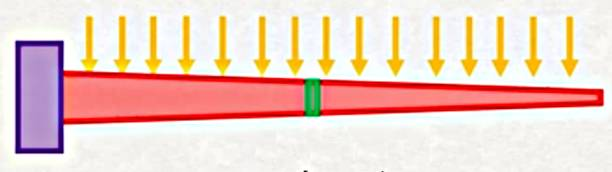
\includegraphics[width=15em]{compscieng_bpp45fem2_02.jpg}

Üstteki resimdeki yeşil bölgeyi düşünelim, o bölgenin iki yan yüzeylerini
düşünürsek, belki soldan sağa giderken biraz değişim olur ama parça çok ufak
olduğu için bu değişim fazla değildir. 

FEM maceramıza çubuk/makaskiriş (bar/truss) öğeleri ile devam edeceğiz.  Bu
yapılar çok basit olmalarına rağmen FEM metadolojisini gösterebilmeleri
açısından uygunlar. Onları sadece küçülme, esneme açısından inceleyeceğiz,
moment, kaykılma gibi konuları şimdilik yok sayacağız. Fakat işleyeceğimiz pek
çok yaklaşım, ``direngenlikleri (stiffness)'' hesaplarken kullandığımız adımlar
her FEM yaklaşımında faydalı olan kavramlar.

Not düşelim, önceki FEM çözümü Galerkin yaklaşımı ile tüm denkleme analitik bir
çözüm buldu. Bu derste ve gerisinde göreceğimiz türden FEM, Galerkin çözümünü
her parçaya uygulayıp ayrıksal sonuçları birleştiriyor.

Makaskiriş alttaki gibi olsun, onu parçalara bölelim, sarı noktalar düğümler
(nodes), düğümleri birleştiren öğeler (elements) var. Bu yaklaşımda yer
değişimleri tüm nesne için değil, her düğümde hesaplayacağız. Yer değişimleri
birbiriyle bağlayan şeyler ögeler, kırmızı ile görülen parçalar.  Bu öğe
parçaları aslında bir aradeğerlemeyi (interpolation) temsil ediyor olacaklar,
eğer iki düğümün yer değişimini biliyorsam onları bağlayan parçanın yer
değişimini bunları kullanarak, aradeğerleme yaparak hesaplayabilirim.

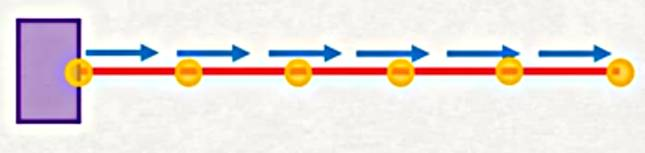
\includegraphics[width=15em]{compscieng_bpp45fem2_03.jpg}

Eğer tek bir öğeye bakarsak,

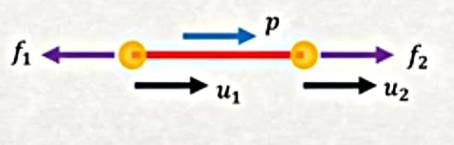
\includegraphics[width=15em]{compscieng_bpp45fem2_04.jpg}

Yer değişimler her düğüm için demiştik, $u_1,u_2$, amacımız onları hesaplamak.
Eğer bu değişimleri hesaplayabilirsem, daha önce belirttiğimiz gibi, aradaki
öğenin yer değişimini yaklaşık olarak, iki uca bağlı olarak hesaplayabilirim.
Yani eğer düğümlerin her değişimini biliyorsam her şeyin yer değişimini
biliyorum demektir.

Galerkin metotuna başlayalım. Metot uygulanınca bize yer değişimleri için bir
direngenlik matrisi ve öğeler için düğümsel kuvvet vektörü vermeli. Her şey
düğümlerde hesaplanıyor dedik, peki sisteme dağıtık bir yük uygulanıyorsa
ne yapacağız? Bu tür kuvvetlerin düğümler arasında etkili olduğunu biliyoruz,
o zaman bu tür kuvvetleri $x,y,z$ bileşenlerine ayırıp onları düğümlere etkili
vektörler haline getirebilirim.

Ana denklemle başlarsak,

$$
E A \frac{\ud^2 y}{\ud X_1^2} = -p
$$

Artık (residual) hesabı şöyle,

$$
R = EA \frac{\ud^2 u}{\ud X_1^2} + p
$$

Bu artığın tanım bölgesi üzerinden ağırlıklı entegralinin sıfır olmasını
istiyoruz,

$$
\int_\Omega R N_i \ud x = 0 
$$

Dikkat, daha önce ağırlık $W_i$ kullanmıştık, şimdi $N_i$ var, bu fonksiyonlar
her düğümde tanımlı şekil fonksiyonu (shape function) olacak. O şekillerin ne
seçildiği FEM'in ana özelliklerinden, detayları göreceğiz.. Şimdi $R$'yi açıp
düzenleme yaparsak,

$$
\int _{0}^{L} \left( EA \frac{\ud^2 u}{\ud X_1^2} + p  \right) N_i \ud X_1 = 0 
$$

$$
\int _{0}^{L} \left( EA \frac{\ud^2 u}{\ud X_1^2} \right) N_i \ud X_1 =
- \int _{0}^{L} p N_i \ud X_1
$$

Parçalı Entegral tekniğini uygulayalım,

$$
\int _{0}^{L} EA \left( \frac{\ud^2 u}{\ud X_1^2}  \right) N_i \ud X_1 =
\left( EA \frac{\ud u}{\ud X_1} N_i \right) \bigg\vert_{X_1=0}^{X_1=L} -
\int_{0}^{L} EA
\left( \frac{\ud u}{\ud X_1} \right)
\left( \frac{\ud N_i}{\ud X_1} \right) \ud X_1 =
- \int _{0}^{L} p N_i \ud X_1
$$

Ekşi işaretler olmasın diye birkaç yer değişimi yapalım,

$$
\int_{0}^{L} EA
\left( \frac{\ud u}{\ud X_1} \right)
\left( \frac{\ud N_i}{\ud X_1} \right) \ud X_1
=
\left( EA \frac{\ud u}{\ud X_1} N_i \right) \bigg\vert_{X_1=0}^{X_1=L} +
\int _{0}^{L} p N_i \ud X_1 
$$

Eşitliğin sağındaki birinci terime dikkat edelim, orada fiziksel anlamı olan bir
ilişki görüyor muyuz? $EA$ çarpı $\ud u / \ud x$.. Tanıdık geliyor mu?  O ifade
aslında bir kuvvet değil mi? Çünkü hatırlarsak $\ud u / \ud x$ yer değişimin
türevi, ki bu gerilme, gerilmeyi Young Genliği $E$ ile çarpınca stres elde
ederim. Ek olarak $A$ ile alan çarpımı var, stres kuvvet bolu alan olduğu için
stresi alanla çarpınca geriye kuvvet kalır. Demek ki o terimle eksenel kuvvet
elde ediyorum, bir düğümde konsantre edilmiş $f = E A \epsilon$ kuvvetini
hesaplıyorum. 





















[devam edecek]

Kaynaklar

[1] Petitt, {\em Intro to the Finite Element Method}, University of Alberta,
    \url{https://www.youtube.com/watch?v=2iUnfPRk6Ro&list=PLLSzlda_AXa3yQEJAb5JcmsVDy9i9K_fi}

\end{document}
